\documentclass{report}

\usepackage{amsmath}
\usepackage{amssymb}
\usepackage{fullpage}
\usepackage[framemethod=TikZ]{mdframed}
\usepackage{lipsum}
\mdfdefinestyle{MyFrame}{%
    linecolor=black,
    outerlinewidth=0.3pt,
    roundcorner=1pt,
    innertopmargin=\baselineskip,
    innerbottommargin=\baselineskip,
    innerrightmargin=20pt,
    innerleftmargin=20pt,
    backgroundcolor=gray!50!white}
\usepackage{listings}
\lstset{basicstyle=\footnotesize}

\lstdefinestyle{custom}{
  belowcaptionskip=1\baselineskip,
  breaklines=true,
  frame=L,
  xleftmargin=\parindent,
  language=Python,
  showstringspaces=false,
  basicstyle=\footnotesize\ttfamily,
  keywordstyle=\bfseries\color{green!40!black},
  commentstyle=\itshape\color{purple!40!black},
  identifierstyle=\color{blue},
  stringstyle=\color{orange},
}

\title{HybGe-Flow3D User Manual, Version 0.0.1}
\author{Timothy B. Costa}

\begin{document}

\maketitle
\tableofcontents

\chapter{HybGe-Flow3D Overview}

HybGe-Flow3D (HGF) is a software package that solves laminar fluid flow problems
in complex geometries and produced upscaled conductivites. This software
is distributed freely AS IS and with ABSOLUTELY NO WARRANTY, and with
the hope that it will be used and extended by the scientific computing community.
In this document we describe how to compile and run Hybge-Flow3D.\\

This software was developed under the partial support of the National Science Foundation,
on the project NSF-DMS 1115827 "Hybrid modeling in porous media."

\section{License \& Citation}

HybGe-Flow3D Copyright (C) Timothy B. Costa.\\

\noindent This program is free software; you can redistribute and/or modify it under the terms
of the GNU General Public License as published by the Free Software Foundation, either
version 3 of the license, or any later version.\\

\noindent This software is distributed AS IS and WITHOUT ANY WARRANTY.\\

\noindent A copy of the GNU General Public License is included in the source and can also be found
at \\ http://www.gnu.org/licenses/.\\

\noindent Publications making use of HybGe-Flow3D should cite this software package. An example citation
is given as:

\begin{mdframed}[style=MyFrame]
  Costa, T., "HybGe-Flow3D", Package Version 0.0.1, http://github.com/costat/HybGe-Flow3D.
\end{mdframed}

\section{Model \& Discretization}

The basic equations solved by HGF are the Stokes equations, modified
with a resistive term corresponding to an immersed boundary representation of complex geometry.
\begin{align*}
  -\mu \nabla^2 u + \frac{1}{\eta}\chi_{\Omega_g} = -\nabla p, \quad &x\in \Omega, \\
  u = u_D, \quad &x\in \partial \Omega_D \\
  \nabla u \cdot n = 0, \quad &x\in \partial \Omega_N.
\end{align*}
Here, $\Omega \subset \mathbb{R}^d$ with $d=3$ or $d=2$ is the simulation domain,
and $\partial \Omega$ is its boundary. $\partial \Omega_D$ refers to the
'Dirichlet boundary' where the fluid velocity is prescribed. This is used
for no-slip and inflow boundary conditions.
$\partial \Omega_N$ refers to the 'Neumann boundary' where a homogeneous diffusive flux
is prescribed. This is used for outflow conditions.
Additionally we have $\Omega = \Omega_g \cup \Omega_f$, $\Omega_g \cap \Omega_f = \emptyset$,
where $\Omega_g$ refers to the immersed boundary and $\Omega_f$ the fluid flow domain.
In these equations $u$ is the fluid velocity, $p$ is the fluid pressure,
and $\mu$ is the fluid viscosity. $\chi_{\Omega_g}$ is the indicator functions
for the immersed boundary domain $\Omega_g$, and $\eta$ is a penalization
parameter, taken to be very small.
HybGe-Flow3D solves the above fluid flow model by a staggered-grid
finite volume discretization.

\chapter{Installation}

HybGe-Flow3D uses the Paralution linear algebra package. In this section
we review the process of building Paralution, installing an environment module file
for Paralution,
and then compiling HybGe-Flow3D on a Linux machine.

\section{Building Paralution}

Paralution 1.0.0 is straightforward to build on Linux machines
using cmake. The instructions contained here can be found at \\
http://www.paralution.com/download/.\\

\noindent First, navigate to the directory in which you will build paralution.
Then grab the tar file containing Paralution.

\begin{mdframed}[style=MyFrame]
\$ wget http://www.paralution.com/downloads/paralution-1.0.0.tar.gz
\end{mdframed}

\noindent The following steps build paralution using cmake.

\begin{mdframed}[style=MyFrame]
  \$ tar zxvf paralution-1.0.0.tar.gz

  \noindent\$ cd paralution-1.0.0

  \noindent\$ mkdir build

  \noindent\$ cd build

  \noindent\$ cmake ..

  \noindent\$ make
\end{mdframed}

\noindent Next we write an environment module file for Paralution.
This file is placed at /usr/share/modulefiles/paralution-1.0.0.

\lstset{style=custom}
\begin{lstlisting}
#%Module 1.0
#
#  Paralution module
#

module-whatis "paralution/1.0.0"

set paralution_home /path/to/paralution/build
prepend-path    PATH                  $paralution_home/bin

prepend-path    LIBRARY_PATH          $paralution_home/lib
prepend-path    LD_LIBRARY_PATH       $paralution_home/lib
prepend-path    CMAKE_LIBRARY_PATH    $paralution_home/lib

prepend-path    INCLUDE_PATH          $paralution_home/inc
prepend-path    C_INCLUDE_PATH        $paralution_home/inc
prepend-path    CPLUS_INCLUDE_PATH    $paralution_home/inc
prepend-path    CMAKE_INCLUDE_PATH    $paralution_home/inc

setenv          PARALUTION_HOME       $paralution_home
setenv          PARALUTION_DIR        $paralution_home
\end{lstlisting}

\noindent Finally, type
\begin{mdframed}[style=MyFrame]
  \$ module avail
\end{mdframed}
and verify that paralution-1.0.0 is an available module.

\section{Building HybGe-Flow3D}

Once paralution is built and a module file is in place, building
HybGe-Flow3D is simple.
First, clone (or download from www.github.com/costat/HybGe-Flow3D/) the repository.
\begin{mdframed}[style=MyFrame]
  \$ cd /path/to/build/hgf

  \noindent\$ git clone git@github.com:costat/HybGe-Flow3D
\end{mdframed}
Then navigate into the repository.
\begin{mdframed}[style=MyFrame]
  \$ cd ./HybGe-Flow3D
\end{mdframed}
Next, load the Paralution module.
\begin{mdframed}[style=MyFrame]
  \$ module load paralution-1.0.0
\end{mdframed}
Finally, execute the compile script.
\begin{mdframed}[style=MyFrame]
  \$ ./compile.bash
\end{mdframed}

\chapter{Running HybGe-Flow3D}

The user needs to interact with two files to simulate a problem.
First, a geometry file needs to be provided. Second,
the boundary conditions and requested output
are handled in the top section of the file stokesolve.py:

\lstset{style=custom}
\begin{lstlisting}
import numpy as np
import time
import sys
import hgf
import re

##############################################################################
### PROBLEM SETUP, USER DEFINES GRID, VISCOSITY, AND NUMBER OF OMP THREADS ###
##############################################################################

# GRID INFORMATION. USER PROVIDES PATH TO .DAT FILE CONTAINING
# VOXEL ARRAY OF 0S 1S AND 2S.
# ALSO,USER PROVIDES TOTAL GRID LENGTHS IN EACH DIRECTION.
gridfiles = './grids/test2d.dat'
L = 1.
W = 1.
H = 1.

# PRINCIPAL FLOW DIRECTION, 0 - X, 1 - Y, 2 - Z, SINGLE FLOW DIRECTION SOLVES,
# PRODUCES CONSTANT K FOR USE IN PORE-NETWORK THROATS
# 3 - ALL DIRECTIONS, PRODUCES UPSCALED K TENSOR
direction = 0

# SET VISCOSITY
visc = 0.001

# NUMBER OF OMP THREADS FOR USE IN PARALUTION LINEAR ALGEBRA
nThreads = 4

##########################################################
### SWIG TRANSLATIONS, USER SHOULD NOT EDIT BELOW HERE ###
##########################################################

.
.
.
\end{lstlisting}

\noindent We see here that the user needs to provide a grid data file,
select total grid dimensions, choose a boundary condition
problem type, set the viscocity, and choose the number of openMP
threads available to Paralution.
In the next two sections we review the details of these choices, beginning
with describing the grid data file.

\section{Problem Geometry}

Solving a problem on a new geometry requires the creation
of a file $<$geometryname$>$.dat. The file contains
a voxel array detailing whether a cell in the geometry
is inactive (not part of the computational domain) or active either
fluid domain or immersed boundary domain.
All geometry files describe a rectangle (in 2D) or a
box (in 3D), but innactive cells are not part of the computational domain,
and are ignored by the gridder.
The following is a very simple
2D example.
\lstset{style=custom}
\begin{lstlisting}
  nx = 21, ny = 13, nz = 0
  1 1 1 1 1 1 1 1 1 0 0 0 1 1 1 1 1 1 1 1 1
  1 1 1 1 1 1 1 1 1 0 0 0 1 1 1 1 1 1 1 1 1
  1 1 1 1 1 1 1 1 0 0 0 0 0 1 1 1 1 1 1 1 1
  1 1 1 1 1 1 0 0 0 0 0 0 0 0 0 1 1 1 1 1 1
  1 1 1 1 0 0 0 0 0 0 0 0 0 0 0 0 0 1 1 1 1
  0 0 0 0 0 0 0 0 0 2 2 2 0 0 0 0 0 0 0 0 0
  0 0 0 0 0 0 0 0 0 2 2 2 0 0 0 0 0 0 0 0 0
  0 0 0 0 0 0 0 0 0 2 2 2 0 0 0 0 0 0 0 0 0
  1 1 1 1 0 0 0 0 0 0 0 0 0 0 0 0 0 1 1 1 1
  1 1 1 1 1 1 0 0 0 0 0 0 0 0 0 1 1 1 1 1 1
  1 1 1 1 1 1 1 1 0 0 0 0 0 1 1 1 1 1 1 1 1
  1 1 1 1 1 1 1 1 1 0 0 0 1 1 1 1 1 1 1 1 1
  1 1 1 1 1 1 1 1 1 0 0 0 1 1 1 1 1 1 1 1 1

\end{lstlisting}

\noindent In this file the first line lists the total number of cells along the x axis, nx,
y axis, ny,
and z axis, nz. For a 2D problem nz is set to 0.
Next the array of 0s 1s and 2s describes the status of each cell in
in the geometry. A cell value of 0 corresponds to the fluid flow domain,
a cell value of 1 corresponds to inactive cells, and a cell value of 2
corresponds to the immersed boundary. So, the example
above correponds to a simple pore geometry with an object blocking
the flow in the center that is enforced by the immersed boundary term.

\section{Problem Selection}

After a geometry file has been created the user must
edit the top section of the file stokesolve.py.
\begin{lstlisting}
##############################################################################
### PROBLEM SETUP, USER DEFINES GRID, VISCOSITY, AND NUMBER OF OMP THREADS ###
##############################################################################

# GRID INFORMATION. USER PROVIDES PATH TO .DAT FILE CONTAINING
# VOXEL ARRAY OF 0S 1S AND 2S.
# ALSO,USER PROVIDES TOTAL GRID LENGTHS IN EACH DIRECTION.
gridfiles = './grids/test2d.dat'
L = 1.
W = 1.
H = 1.

# PRINCIPAL FLOW DIRECTION, 0 - X, 1 - Y, 2 - Z, SINGLE FLOW DIRECTION SOLVES,
# PRODUCES CONSTANT K FOR USE IN PORE-NETWORK THROATS
# 3 - ALL DIRECTIONS, PRODUCES UPSCALED K TENSOR
direction = 0

# SET VISCOSITY
visc = 0.001

# NUMBER OF OMP THREADS FOR USE IN PARALUTION LINEAR ALGEBRA
nThreads = 4

\end{lstlisting}

\noindent First, the geometry file location is given in line 16,
\begin{lstlisting}
  gridfiles = './path/to/<geometryname>.dat'
\end{lstlisting}

\noindent Second the total dimensions of the geometry need to be given. Note
that these values correspond to the total length of the box or rectangle, including
inactive cells. L is the length in the x direction, W is the width in the y
direction, and H is the height in the z direction. For a 2D problem H
may be set to any value, as the nz = 0 term in the geometry file informs
the solver that the problem is in 2D.\\

\noindent Next the the boundary condition setup is determined by setting
the integer 'direction' in line 24. This integer is set to a value
of 0, 1, 2, or 3, which corresponds to the following flow problems:
\begin{itemize}
  \item direction = 0 $\rightarrow$ inflow on x min wall, outflow on x max wall,
        no slip everywhere else.
  \item direction = 1 $\rightarrow$ inflow on y min wall, outflow on y max wall,
        no slip everywhere else.
  \item direction = 2 $\rightarrow$ inflow on z min wall, outflow on z max wall,
        no slip everywhere else.
  \item direction = 3 $\rightarrow$ solves directions 0, 1, and 2 (0 and 1 in 2D)
        so that a full upscaled hydraulic conductivity tensor can be computed.
\end{itemize}

\noindent Next the user sets the fluid viscosity in line 27. Finally, the user tells
the software how many openMP threads to use in the Paralution package.

\section{Simulation \& Output}

Now that the top section of stokesolve.py has been set up, the code
is executed simply by
\begin{mdframed}[style=MyFrame]
\$ python stokesolve.py
\end{mdframed}
Here is an example terminal output from solving the x-flow problem
on the test geometry 'test3d.dat' on a single sandy bridge core.
\begin{mdframed}[style=MyFrame]
\footnotesize
\$ python stokesolve.py
\\

\noindent \hspace{.1cm} Total grid generation time: 2.82711696625
\\

\noindent \hspace{.1cm} Solving the stationary Stokes problem...
\\

\noindent \hspace{.1cm} This version of PARALUTION is released under GPL.

\noindent \hspace{.1cm} By downloading this package you fully agree with the GPL license.

\noindent \hspace{.1cm} Number of CPU cores: 1

\noindent \hspace{.1cm} Host thread affinity policy - thread mapping on every core

\noindent \hspace{.1cm} Number of CPU cores: 1

\noindent \hspace{.1cm} PARALUTION ver B1.0.0

\noindent \hspace{.1cm} PARALUTION platform is initialized

\noindent \hspace{.1cm} Accelerator backend: None

\noindent \hspace{.1cm} GMRES(30) solver starts, with preconditioner:

\noindent \hspace{.1cm} ILU(1) preconditioner

\noindent \hspace{.1cm} ILU nnz = 58968

\noindent \hspace{.1cm} IterationControl criteria: abs tol=1e-15; rel tol=1e-06; div tol=1e+08; max iter=1000000

\noindent \hspace{.1cm} IterationControl initial residual = 0.298187

\noindent \hspace{.1cm} IterationControl RELATIVE criteria has been reached: res norm=1.2121e-07; rel val=4.06488e-07; iter=21

\noindent \hspace{.1cm} GMRES(30) ends

\noindent \hspace{.1cm} Done. Total time: 0.323477983475

\end{mdframed}

\noindent After a simulation is run, there will be two types of output files
in the HGF directory.\\

\noindent If a single flow direction is solved, these files will
be flowrun.dat,
and and one of Kconstant<X,Y,Z>.dat, depending on the flow direction.\\

\noindent The file flowrun.dat contains everything necessary for visualizing
the solution: each component of the velocity, the pressure,
a list of cells in the immersed boundary (for blanking) and
mesh information. The format of the file is written to be easily
loaded into Tecplot for visualization, but Paraview (free) is also
possible.\\

\noindent The file KConstant$\langle$X,Y,Z$\rangle$.dat contains the constant conductivity
computed from the solution.\\

\noindent If all flow directions are solved (direciton = 3 in stokesolve.py) then
7 files are produced. These are flowrun$\langle$X,Y,Z$\rangle$.dat,
KConstant$\langle$X,Y,Z$\rangle$.dat and
KTensor.dat. These files contains the solutions from each solution, the constant
conductivities from each solution, and the upscaled conductivity tensor, respectively.

\chapter{Examples}

\noindent The following examples are found in the included directory /path/to/hgf/grids/.\\

\noindent We begin with a simple problem: Poiseuille flow in a pipe. Figure~\ref{fig:2dpflow}
shows the pressure and x-component of the velocity for the 2d case. Figure~\ref{fig:3dpflow}
shows the pressure and x-component of the velocity for the 3d case.

\begin{figure}
  \centering
  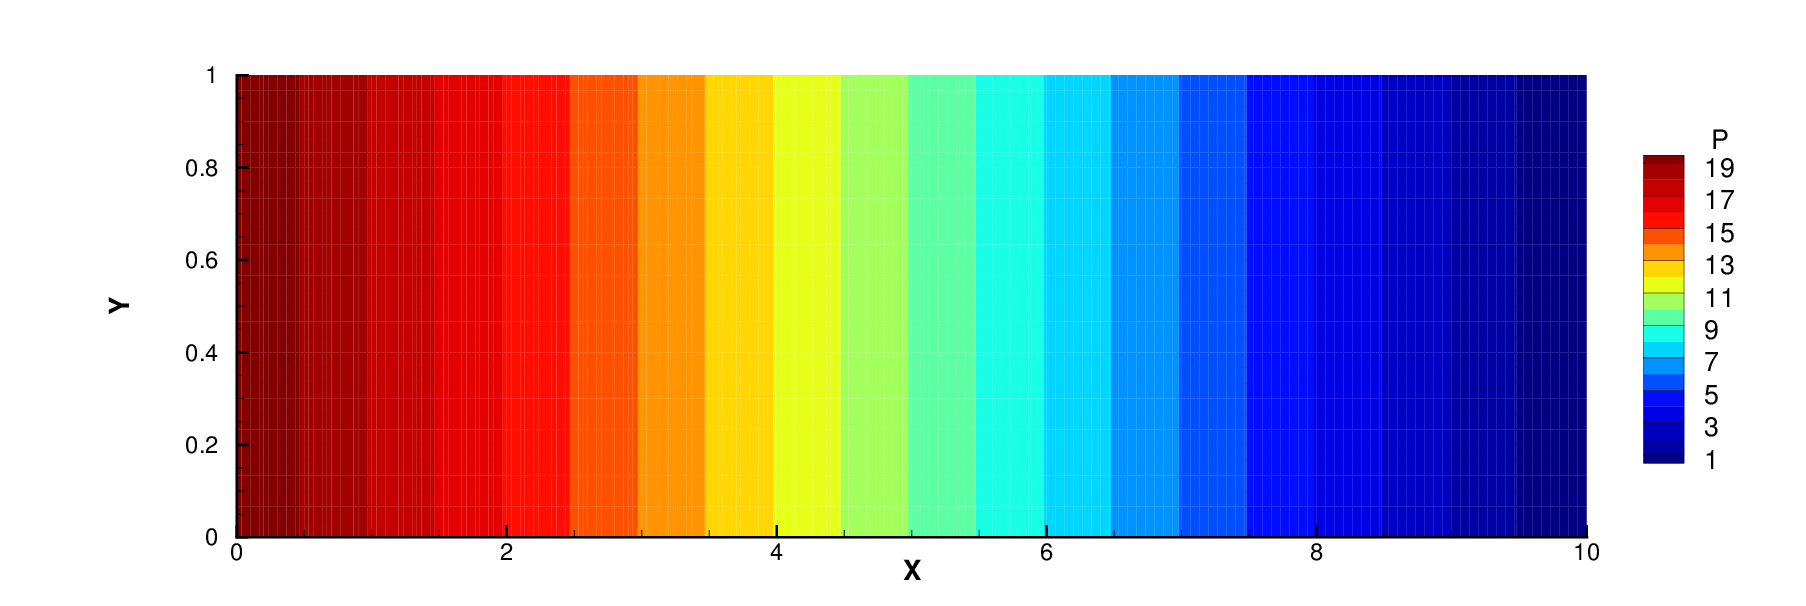
\includegraphics[width=.9\textwidth]{images/pflow2dP.png}\\
  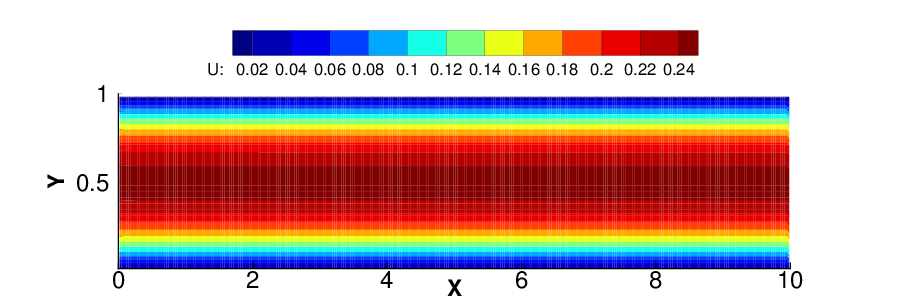
\includegraphics[width=.9\textwidth]{images/pflow2dU.png}
  \caption{\label{fig:2dpflow}Poiseuille flow in a 2D pipe.}
\end{figure}
\begin{figure}
  \centering

  \caption{\label{fig:3dpflow}Poiseuille flow in a 3D pipe.}
\end{figure}
\end{document}
